\begin{figure}[h]
\centering
% KPH
  \begin{subfigure}[b]{0.32\textwidth}
    \includegraphics[width=\textwidth]{safe/carSpeedKph}
  \end{subfigure}%
  ~
  \begin{subfigure}[b]{0.32\textwidth}
    \includegraphics[width=\textwidth]{speed/carSpeedKph}
  \end{subfigure}%
   ~
  \begin{subfigure}[b]{0.32\textwidth}
    \includegraphics[width=\textwidth]{rally/carSpeedKph}
  \end{subfigure}\\
% Corner
  \begin{subfigure}[b]{0.32\textwidth}
    \includegraphics[width=\textwidth]{safe/corner}
  \end{subfigure}%
  ~
  \begin{subfigure}[b]{0.32\textwidth}
    \includegraphics[width=\textwidth]{speed/corner}
  \end{subfigure}%
   ~
  \begin{subfigure}[b]{0.32\textwidth}
    \includegraphics[width=\textwidth]{rally/corner}
  \end{subfigure}\\
% lateralVelocity
  \begin{subfigure}[b]{0.32\textwidth}
    \includegraphics[width=\textwidth]{safe/lateralVelocity}
  \end{subfigure}%
  ~
  \begin{subfigure}[b]{0.32\textwidth}
    \includegraphics[width=\textwidth]{speed/lateralVelocity}
  \end{subfigure}%
   ~
  \begin{subfigure}[b]{0.32\textwidth}
    \includegraphics[width=\textwidth]{rally/lateralVelocity}
  \end{subfigure}\\  
% frontSensor
  \begin{subfigure}[b]{0.32\textwidth}
    \includegraphics[width=\textwidth]{safe/frontSensor}
    \caption{Veilig}
    \label{fig:safe_in}
  \end{subfigure}%
  ~
  \begin{subfigure}[b]{0.32\textwidth}
    \includegraphics[width=\textwidth]{speed/frontSensor}
    \caption{Snel}
    \label{fig:speed_in}
  \end{subfigure}%
   ~
  \begin{subfigure}[b]{0.32\textwidth}
    \includegraphics[width=\textwidth]{rally/frontSensor}
    \caption{Drift}
    \label{fig:drift_in}
  \end{subfigure}\\ 
\caption{Lidmaatschapfuncties invoer}\label{fig:lidfties_in}
\end{figure}

\begin{figure}[h]
\centering
% Accel
  \begin{subfigure}[b]{0.32\textwidth}
    \includegraphics[width=\textwidth]{safe/acceleration}
  \end{subfigure}%
  ~
  \begin{subfigure}[b]{0.32\textwidth}
    \includegraphics[width=\textwidth]{speed/acceleration}
  \end{subfigure}%
   ~
  \begin{subfigure}[b]{0.32\textwidth}
    \includegraphics[width=\textwidth]{rally/acceleration}
  \end{subfigure}\\
% Brake
  \begin{subfigure}[b]{0.32\textwidth}
    \includegraphics[width=\textwidth]{safe/brake}
  \end{subfigure}%
  ~
  \begin{subfigure}[b]{0.32\textwidth}
    \includegraphics[width=\textwidth]{speed/brake}
  \end{subfigure}%
   ~
  \begin{subfigure}[b]{0.32\textwidth}
    \includegraphics[width=\textwidth]{rally/brake}
  \end{subfigure}\\
% steering
  \begin{subfigure}[b]{0.32\textwidth}
    \includegraphics[width=\textwidth]{safe/steering}
  \end{subfigure}%
  ~
  \begin{subfigure}[b]{0.32\textwidth}
    \includegraphics[width=\textwidth]{speed/steering}
  \end{subfigure}%
   ~
  \begin{subfigure}[b]{0.32\textwidth}
    \includegraphics[width=\textwidth]{rally/steering}
  \end{subfigure}\\
% scanAngle
  \begin{subfigure}[b]{0.32\textwidth}
    \includegraphics[width=\textwidth]{safe/scanAngle}
    \caption{Veilig}
    \label{fig:safe_out}
  \end{subfigure}%
  ~
  \begin{subfigure}[b]{0.32\textwidth}
    \includegraphics[width=\textwidth]{speed/scanAngle}
    \caption{Snel}
    \label{fig:speed_out}
  \end{subfigure}%
   ~
  \begin{subfigure}[b]{0.32\textwidth}
    \includegraphics[width=\textwidth]{rally/scanAngle}
    \caption{Drift}
    \label{fig:drift_out}
  \end{subfigure}\\
\caption{Lidmaatschapfuncties uitvoer}\label{fig:lidfties_out}
\end{figure}